\chapter{提案アプローチ}
本論文の問題はニューロンのクラスタリングである.
隣接行列$\bar{A}(X, \mathcal{K}) \in [0, 1]^{I \times I}$をクラスタリングする問題を解く.
ただし,$I$はニューロン数で$\bar{A}(X, \mathcal{K})$の$(i,j)$要素はデータ$X$が与えられた時のニューロン$i$と$j$の結合確率である.
また,$\mathcal{K}$はグループ数の集合である.
本章では$\bar{A}$の推定方法とクラスタリング手法の説明をする.

$\bar{A}$は非負行列因子分解(NMF)とバギングを用いて推定する.
NMFを使う理由は数理モデルに基づいており,次節で説明する.
クラスタリング手法にはスペクトラルクラスタリングを用いる.
スペクトラルクラスタリングはグラフカットとして解釈でき,$\bar{A}$をクラスタリングするのに適している.

\section{隣接行列の推定}
% 本節ではNMFとブートストラップ法によって類似度$A$を推定する方法を述べる.
% NMFで推定するのは$A^* \in \{0,1\}^{I \times I}$であり,$a^*_{ij}$はニューロン$i$とニューロン$j$が同じグループに所属するか否かを表す.
% ブートストラップ法を用いて類似度$A = E[A^* | X]$を推定する.
% $A$の要素$a_{ij}$はニューロン$i$とニューロン$j$が同じグループである確率$Pr(a_{ij} = 1)$を意味する.

\subsection{数理モデル}
カルシウムイメージングデータに対していくつかの仮定をおいた.
\\ \\
\noindent \textbf{仮定 1}\\
グループが$K$個存在し,同じグループ内のニューロンは同時に活動する.
ニューロンは複数のグループに所属することができる.
観測時間内ではグループに属するニューロンは変化しない.
\\ \\
\textbf{仮定 2}\\
複数のグループが同時に活動する時,属するニューロンは被らない(ニューロンが属するグループは同時には活動しない).
\\

これらの仮説をもとに,数理モデルを構築する.
観測データ$X$は$X \in \mathbb{R}_+^{I \times J}$とする.
ただし,$\mathbb{R}_+$を非負の実数の集合,$J$を観測時系列の長さとする.
ある行列$A$の$i$行を$a_{i:}$,$j$列を$a_{:j}$,$(i,j)$要素を$a_{ij}$または$[A]_{ij}$と表記する.
よって,ニューロン$i$の観測時系列は$x_{i:} \in \mathbb{R}_+^{J}$である.

$c_{k:} \in \mathbb{R}^J_+$ ($k=1,\dots,K$)をグループ$k$の活動の時系列とすると,仮定より$x_{i:}$は$c_{i:}$の重み付き和として表す:
\begin{equation}
	x_{i:} = \sum_{k=1}^K d_{ik} c_{k:} + \eta_{i:},
  \label{eq:x}
\end{equation}
ただし,$d_{ik} \in \mathbb{R}^+$で,$\eta_{i:} \in \mathbb{R}^J$はi.i.d.なガウスノイズの時系列である.
カルシウムイメージングのノイズはポアソン分布に従う光子ノイズであるが,光子数が多い場合はガウス分布で近似できる~\cite{Sjulson2007}.

仮定2を置くことによって,\eqref{eq:x}の線形モデルを考えることができる.
仮定2がない場合,あるニューロンの蛍光強度は複数グループからの影響によって上限なく上昇できてしまう.
実際は,ニューロンの蛍光強度の最大値は蛍光タンパク質の量で決まるため,蛍光強度は最大値で飽和する.
その場合\eqref{eq:x}には飽和を組み込まなければいけない.
本論文では,複数グループが同時に活動する場合はそれらも同じグループとみなし,単純な線形モデルで表す.

\eqref{eq:x}は行列形式で以下のように表現できる:
\begin{align}
  % Y &= DC, \\
  X &= DC + H. \label{eq:model_matrix}
\end{align}
ただし,$D \in \mathbb{R}_+^{I \times K}$, $C \in \mathbb{R}_+^{K \times J}$, $H \in \mathbb{R}^{I \times J}$である.
また,$D$の要素$(i,k)$は$d_{ik}$,$C$の$i$行は$c_{i:}$,$H$の$i$行は$\eta_{i:}$である.
NMFのモデルを\Figref{fig:nmf}に示す.

\begin{figure}[htbp]
	\centering
	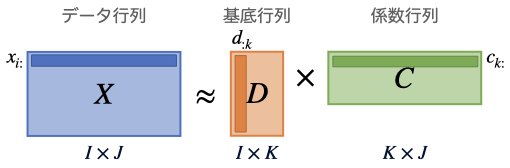
\includegraphics[width=0.8\hsize]{nmf}
	\caption{NMFのモデル.}
	\label{fig:nmf}
\end{figure}

\subsection{NMFによる$\hat{A}$の推定}
非負行列因子分解(nonnegative matrix factorization; NMF)\cite{Lee1999}は行列分解の手法の一つである.
NMFは非負行列を2つの非負行列の積として分解する:
\begin{equation}
	X \approx DC.
\end{equation}
$X$,$D$,$C$は上述の行列であり,\eqref{eq:model_matrix}はNMFの問題として解くことができる.
$D$と$C$を求めるためにNMFでは以下の最適問題を解く:
\begin{equation}
	\argmin_{D \geq 0, C \geq 0} ||X - DC||_F^2.
\end{equation}
基底数$K$は事前に決めなければいけないパラメータである.

NMFの寄与率行列$P \in [0,1]^{I \times K}$の要素を次のように定義する:
\begin{align}
	p_{ik} &= \frac{||d_{ik} c_{k:}||_1}{\sum_{l=1}^K || d_{il} c_{l:} ||_1}.
	% &= \frac{d_{ik} || c_{k:} ||_1}{ \sum_{l=1}^K d_{il} || c_{l:} ||_1 }.
\end{align}
また,概念図を\Figref{fig:kiyoritu}に示す.
\begin{figure}[htbp]
	\centering
	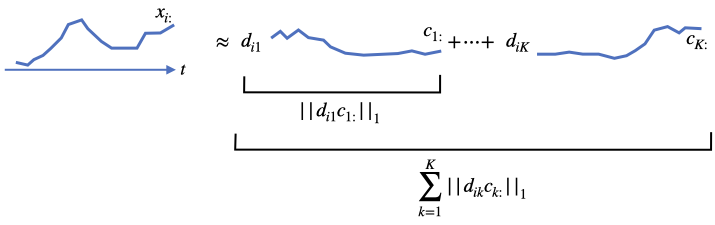
\includegraphics[width=\hsize]{kiyoritu}
	\caption{寄与率の概念図.}
	\label{fig:kiyoritu}
\end{figure}
ニューロン$i$の観測系列$x_{i:}$は$d_{ik}c_{k:} \ (k=1,\cdots,K)$で再構成されている.
観測系列は非負なので,$||d_{ik}c_{k:}||_1$は基底$k$の情報が$x_{i:}$の再構成のうちどれくらいを占めているかを示す.
よって,要素$p_{ik}$は,ニューロン$i$の観測系列$x_{i:}$の再構成にどれくらい基底$k$が寄与したかという量である.
NMFの目的関数に$C$の行和が1という制約を入れると$P=D$となる.

NMFでの推定量$\hat{A}(X,K) \in \{0,1\}^{I \times I}$とする.
$\hat{A}(X,K)$は寄与率行列$P$から作成する.
まず,$P$と同じサイズの行列$G \in \{0, 1\}^{I \times K}$を作る.
$G$は,$P$の各行について最大値のみを$1$,それ以外を$0$とした行列である.
\begin{align}
	g_{ij} = \begin{cases}
		1 & (j = \argmax_{j}p_{ij}) \\
		0 & (\text{otherwise})
	\end{cases}
\end{align}
% まず,以下の手順で$P$と同じサイズの行列$G \in \{0, 1\}^{I \times K}$を作る.
% $p_{i:}$の累積寄与率を$F_i$とおく.
% $F_i$は$p_{i:}$を大きい順に足した関数である.
% 閾値を$threshold$とおき,$F_i < threshold$となる$p_{i:}$のインデックスを$index$とおく.
% $p_{i:}$に該当する$g_{i:}$を
% \begin{align}
% 	g_{ij} = \begin{cases}
% 		1 & (j \in index) \\
% 		0 & (otherwise)
% 	\end{cases}
% \end{align}
% と定義する.

推定量$\hat{A}(X,K)$を
\begin{align}
	\hat{A}(X,K) = G G^{\top},
\end{align}
と定義する.
これより$\hat{A}$は対称行列で,要素$\hat{a}_{ij}$はニューロン$i$とニューロン$j$が同じ基底に所属していたら$1$,していなかったら$0$となる.

この推定量はcluster ensembleでも用いられているpairwise similarity\cite{Boongoen2018}と似たものになっている.

\subsection{バギング}
アンサンブル学習の一つにバギング\cite{Breiman1996}がある.
バギングはある予測器にブートストラップサンプルを入力して,その結果の平均を用いることで精度を向上させる方法である.
ブートストラップ法\cite{Efron1979}とは,推定量の分布を近似する方法である.
ブートストラップ法によって$X$が与えられた時の$\hat{A}(X,K)$の分布を近似することができる.
% データ$X$が分布$F$に従うとき,確率変数$R(X,F)$を推定する問題を考える.
% ブートストラップサンプル$X^*$を作成して,$R^* = R(X^*, \hat{F})$を推定すると,$R^*$の分布は$R$の分布を近似する.
% $F = \hat{F}$の時,$R^*$と$R$の分布は一致する.

提案アプローチではブートストラップサンプル$\{X^{*b}; b = 1, \dots, B\}$からNMFを用いて$\hat{A}^{*b} = \hat{A}(X^{*b},K)$を推定する.
これより$\hat{A}^*$の分布が求まるので,$\hat{a}^*_{ij}$が$1$となる確率が以下のようにして求まる:
\begin{align}
	Pr(\hat{a}^*_{ij} = 1) = E[\hat{a}^*_{ij}|X].
\end{align}

クラスタリングに用いる隣接行列$\bar{A}(X,\mathcal{K})$を$\hat{A}^*$の期待値$E[\hat{A}^*]$として推定する:
\begin{align}
	\bar{A}(X,\mathcal{K}) &= \frac{1}{B} \sum_{b=1}^B A^{*b}, \\
	\mathcal{K} &= \{K\}.
\end{align}
$\mathcal{K}$は要素が$K$の集合という表記にしているが,これは後述するモデル平均のためである.

ブートストラップサンプルの作成にはいくつかの方法が考えられる.
簡単な3種類の方法について説明する.
列のサンプリングによるブートストラップは,データ行列$X$の各列がデータサンプルとしてみなせるので,列をサンプリングして$X^{*b}$を作る方法である.
% \begin{align}
% 	X^* = \left[ X_{:sample(1,\dots,J)}, \cdots, X_{:sample(1,\dots, J)}\right],
% \end{align}
ブロックブートストラップでは,複数列を塊としてサンプリングする.
この方法は時系列データでのブートストラップで用いられており,時間方向に制約の入ったNMFなどでは有効である.
残差型ブートストラップは一回NMFのモデルを推定し,推定後の残差をサンプリングして推定した$DC$に足す方法である.
\begin{align}
	X^{*b} = \hat{D} \hat{C} + H^{*b},
\end{align}
ただし,$\hat{D}$と$\hat{C}$は最優推定量で,$H^{*b}$は$X - \hat{D}\hat{C}$をリサンプリングした行列である.
ニューロンごとにノイズの大きさが異なることが想定される場合は,行ごとにリサンプリングを行うのが適切だと考えられる.
NMFのモデル\eqref{eq:model_matrix}では$H$はi.i.d.なノイズという仮定を置いているので,残差型ブートストラップが一番モデルに沿ったブートストラップ方法と言える.

機械学習の分野でブートストラップ法が多く使われる場面はバギング\cite{Breiman1996}である.
バギングとは,ブートストラップ法によって学習器を増やしその出力の平均をとる学習方法である.
今回のブートストラップ法の使い方もバギングとして見ることができる.

\subsection{NMFの基底数}
NMFの基底数の決め方にはいくつかのアプローチがある.
まずは,専門家や解析者の知識に基づいて決めることである.
この方法はデータに対して十分な知識がない時には使えない.

次にBIC~\cite{wasserman2000a}やAIC~\cite{Akaike1974}を用いる方法である.
これらは漸近理論に基づいた近似を行った情報量基準である.
NMFはデータが増えるほどパラメータ数$(I + J) * K$が増えるという特徴があり,これらを用いるのは本来不適切である.

次にRのNMFパッケージにも組み込まれているBrunetら~\cite{Brunet2004}の方法を紹介する.
彼らはNMFの推定結果からノード同士が同じ基底に所属するかしないかを表すconnectivity matrix $M \in \{0, 1\}^{I \times I}$を作成する.
本論文の推定量$A$と同じ意味の行列である.
初期値を20-100回変化させて$M$の平均$\bar{M} \in [0, 1]^{I \times I}$を計算する.
彼らは真の基底数ではこの推定量が$0$か$1$に寄るようになると仮定して,最も$\bar{M}$が安定する基底数を求める.
安定度は$1- \bar{M}$とそのcophenetic correlation coefficientのPearson correlationから計算する.

Ubaruら~\cite{Ubaru2017}はブートストラップを用いてNMFを行っており,$D$がそれほど変わらない基底数を採用している.
推定した$D^{*b}$同士の相互相関行列についてdissimilarity~\cite{Wu}を測りその平均が最小となる基底数を用いる.

Hutchinsらはテストデータに対するRSS(residual sum of squares)が真の基底数以降になるとあまり下がらなくなると論じている\cite{Hutchins2008}.

Bayesian NMFではギブスサンプリングなどを用いてモデルエビデンスを計算している\cite{Cemgil2009}.

上記で述べた方法の他にも様々な方法が考案されているが,全てのデータに当てはめられるような枠組みは存在しない.

\subsection{モデル平均}
モデル平均とは異なるモデルの推定量の平均をとって精度向上を測る方法である.
$\bar{A}$は基底数によって行列サイズが変化しないので,異なる基底数の推定結果の平均をとることができる.
その場合の推定量は:
\begin{align}
	\bar{A}(X,\mathcal{K}) &= \frac{1}{|\mathcal{K}|} \sum_{k \in \mathcal{K}} \frac{1}{B} \sum_{b=1}^B \hat{A}(X^{*b}, k),\\
	\mathcal{K} &= \{K_{min}, \dots, K_{max}\},
\end{align}
ただし,平均する最小の基底数を$K_{min}$,最大の基底数を$K_{max}$とする.
Bayesian model averagingを用いて事後確率による重み付けも検討したがうまくいかなかった.
概要は5章で述べる.

NMFの基底数を求めるのは難しい問題なので,モデル平均によって,異なる基底数の推定結果を平均して精度をあまり落とさないようにする.
今回扱うデータから推定される$\hat{A}$は基底数が異なる時に大きくは変化しないと考えられる.
% 真の基底数周りで平均した$A$の方が真の基底数でないモデルから推定された$A_k$よりも精度が落ちないと考えられる.

アンサンブル学習では,それぞれのモデルにある程度の推定精度があり\cite{Kittler1998},答えに多様性がある方が精度が上がる\cite{Kuncheva2006}と言われている.
本論文での使い方は異なり,真の基底数が分からない時に推定結果をなまして推定を間違うリスクを下げるという使い方である.

\subsection{NMFの一意性}
NMFの推定には一意性がなく,ある正則行列$Q$を考えた時,
\begin{align}
	X &= DC \\
	&= D Q R C \label{eq:dqrc} \\
	&= D'C', \\
	R &= Q^{-1}, \\
	D' &= DQ, \\
	C' &= RC,
\end{align}
のように別の$D'$と$C'$が推定される可能性がある.

NMFに一意性がある条件は\cite{Fu}などでまとめられている.
しかし,一意性を持たせるにはかなり条件が狭められる.

NMFと同じように非負行列を分解する手法にnonnegative rank factorization (NRF)~\cite{Dong2014}がある.
NRFではデータ行列$X$を$X = DC$に分解できる最小の基底数をnonnegative rank $\text{rank}_+(X)$と定義し,$\text{rank}(X) = \text{rank}(X)_+$となる行列$X$を対象とする.
全ての非負行列はNMFできるが,NRFができるとは限らない.
NRFの計算はNP困難であるが,\cite{Dong2014}ではNRFの計算と,NRFを持たない行列に対してMNRSという分解の計算方法を提示している.
しかし,$X$にノイズが乗っている場合にNRFが存在する条件は調査されていない.

\eqref{eq:dqrc}の場合の$D'$と$C'$を用いて作られる寄与率行列$P'$と元の寄与率行列$P$の関係を考える.
% 要素$p'_{ik}$の分子は,$D'$と$C'$が正であることを用いて
% \begin{align}
% 	d'_{ik} ||c'_{k:}||_1 &= \left( \sum_{l = 1}^K d_{il} q_{lk} \right) \left( \sum_{m = 1}^K r_{km} ||c_{m:}||_1 \right) \\
% 	&= \sum_{m = 1}^K \left( d_{i1} q_{1k} r_{km} + \cdots + d_{iK} q_{Kk} r_{km} \right) ||c_{m:}||_1,
% \end{align}
% である.
% 分母を考えると,
% \begin{align}
% 	\sum_{l=1}^K d'_{il}||c'_{l:} ||_1 &= \sum_{l = 1}^K \sum_{m = 1}^K \left( d_{i1} q_{1l} r_{lm} + \cdots + d_{iK} q_{Kl} r_{lm} \right) ||c_{m:}||_1 \\
% 	&= \sum_{m = 1}^K \left( d_{i1} \sum_{l = 1}^K q_{1l}r_{lm} + \cdots d_{iK} \sum_{l = 1}^K q_{Kl} r_{lm}\right) ||c_{m:}||_1
% \end{align}
% \eqref{eq:dqrc}より,
% \begin{align}
% 	\sum_{l = 1}^{K} q_{il} r_{lj} = \begin{cases}
%     1 & (i = j) \\
%     0 & (otherwise)
%   \end{cases}
% \end{align}
% なので,
% \begin{align}
% 	\sum_{l=1}^K d'_{il} || c'_{l:} ||_1 &=& \sum_{m = 1}^K d_{im} ||c_{m:}||_1,
% \end{align}
% となり,$p_{ik}$と$p'_{ik}$の分母は一致する.
% 寄与率$p'_{ik}$は,
% \begin{align}
% 	p'_{ik} &= \frac{ d'_{ik} || c'_{k:}||_1 }{ \sum_{m = 1}^K d'_{im} || c'_{m:}||_1 } \\
% 	&= \frac{\sum_{l = 1}^K d_{il} q_{lk}}{\sum_{m=1}^K d_{im} || c_{m:} ||_1} ||c'_{k:}||_1 \\
% 	&= ||c'_{k:}||_1 \sum_{l = 1}^K \frac{d_{il}}{\sum_{m=1}^K d_{im} || c_{m:} ||_1} q_{lk} \\
% 	p_{il} = \frac{d_{il} ||c_{l:}||_1 }{ \sum_{m = 1}^K d_{im} || c_{m:} ||_1 } \text{より,} \\
% 	&= ||c'_{k:}||_1 \sum_{l = 1}^K \frac{p_{il}}{ ||c_{l:}||_1 } q_{lk}\\
% 	&= \sum_{l = 1}^K \frac{ ||c'_{k:}||_1 }{ ||c_{l:}||_1 } q_{lk} p_{il}
% \end{align}
% となる.
% これより,
% \begin{align}
% 	P' &= PV, \\
% 	V &\in \mathbb{R}^{K \times K}, \\
% 	v_{ij} &= \frac{ || c'_{j:} ||_1 }{|| c_{i:} ||_1} q_{ij},
% \end{align}
% と表せることから,$P'$は$P$を変換した行列であることがわかる.
% この変換によって異なるニューロンの寄与率は同じだけ変化する.
簡単のため,$X$に行和$1$の正規化を加え$C$に行和$1$の制約を加える.
この時$D$の行和も$1$となり,$P = D$となる.
\eqref{eq:dqrc}より,$P' = PQ$となる.
この時,$G$の作り方には一意性がないため推定量$A$にも一意性がない.

$K=3$の場合の図を用いて説明をする.
\Figref{fig:d-space}に$C$の空間内の$x_{i:}$と$D$の空間内の$d_{i:}$を表す.
$d_{i:}$の和は$1$であるが,軸は\Figref{fig:d-rotate}のように動くことができる.
$G$を作成した際にニューロンがどの基底に所属するかを\Figref{fig:p-rotate}に示した.
軸の変化によってニューロンが所属する基底が変化することがある.
その結果,推定量$\hat{A}$も変化するため,NMFは$\hat{A}$の推定に関して一意性はない.
第3章の実験を通して一意性がなくても精度に向上は見られることを確かめる.

\begin{figure}[htbp]
    \begin{minipage}{0.69\hsize}
			\begin{center}
					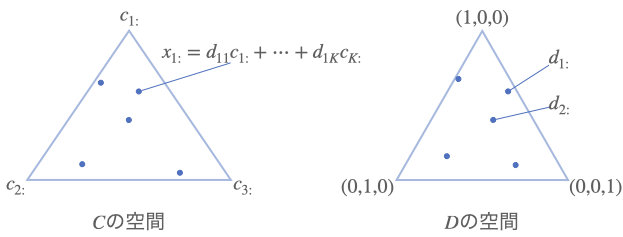
\includegraphics[width=\hsize]{d-space}
					\caption{$C$の空間と$D$の空間.}
					\label{fig:d-space}
			\end{center}
		\end{minipage}
    \begin{minipage}{0.3\hsize}
			\begin{center}
					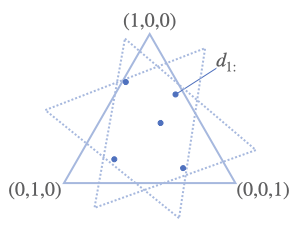
\includegraphics[width=\hsize]{d-rotate}
					\caption{変換$Q$によって$D$の空間の軸は回転・移動する.}
					\label{fig:d-rotate}
			\end{center}
		\end{minipage}
\end{figure}
\begin{figure}[htbp]
		\begin{center}
				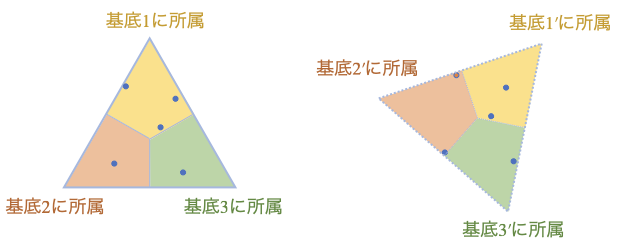
\includegraphics[width=0.8\hsize]{p-rotate}
				\caption{$D$の空間の軸の変化によってニューロンが所属する基底が変化する.}
				\label{fig:p-rotate}
		\end{center}
\end{figure}


\section{$\bar{A}$を用いたクラスタリング}
$\bar{A}$のクラスタリングにはスペクトラルクラスタリングを用いる.
スペクトラルクラスタリングは,隣接行列からグラフラプラシアンを求め,その固有ベクトルをk-meansなどでクラスタリングする.
他のクラスタリング手法も使えるが,$\bar{A}$をグラフとして見ることができるため,スペクトラルクラスタリングを用いる.

\subsection{スペクトラルクラスタリングのクラスタ数の決め方}
クラスタ数の決め方には様々な方法がある.
クラスタリング手法によらない方法には,安定性を見る方法\cite{Ben-Hur}やGap統計量\cite{Tibshirani}がある.
スペクトラルクラスタリングに特化した方法としては,固有値ギャップを見る方法\cite{VonLuxburg}がある.
固有値ギャップは固有値を小さい順にプロットした際に,一気に固有値が大きくなる箇所であり,その順位をクラスタ数とする.

クラスタ数が明瞭な類似度行列について固有値ギャップとGap統計量を試した結果,固有値ギャップの方が安定してクラスタ数を決定できたため,固有値ギャップを用いる.
固有値ギャップは目で見て判断しなければならないが,本実験では固有値の差分を取って大津の二値化にかけ,差分の大きいグループの最大固有値の順位を固有値ギャップとして計算する.

\subsection{評価}
クラスタリングの評価方法には\cite{Molter2018}で用いられていたBest Match scoreを用いる.
二つのクラスタリング結果$\mathcal{B} = \{B_1, \dots, B_{|\mathcal{B}|}\}$と$\mathcal{B^\prime} = \{B^\prime_1, \dots, B^\prime_{|\mathcal{B}^\prime|}\}$があった場合を考える.
ただし,$B_k$はクラスタ$k$に所属するニューロンの集合である.
Best Match scoreは
\begin{align}
	\text{Best Match score} = \frac{1}{|\mathcal{B}| + |\mathcal{B^\prime}|} \left( \sum_{B \in \mathcal{B}} \max_{B^\prime \in \mathcal{B^\prime}} \frac{|B \cap B^\prime|}{|B \cup B^\prime|} + \sum_{B^\prime \in \mathcal{B^\prime}} \max_{B \in \mathcal{B}} \frac{|B \cap B^\prime|}{|B \cup B^\prime|} \right),
\end{align}
である.
これはJaccard係数のクラスタ数の平均である.
2つのクラスタリング結果が近いほどBest Match scoreは高くなる.
評価には$\mathcal{B}$をクラスタリング結果,$\mathcal{B}^\prime$を真のクラスタ集合として計算する.
